% !TeX spellcheck = en_GB
% !TeX program = pdflatex
%
% LuxSleek-CV 1.1 LaTeX template
% Author: Andreï V. Kostyrka, University of Luxembourg
%
% 1.1: added tracking and letter-spacing for prettier lower caps, added `~` for language levels
% 1.0: initial release
%
% This template fills the gap in the available variety of templates
% by proposing something that is not a custom class, not using any
% hard-coded settings deeply hidden in style files, and provides
% a handful of custom command definitions that are as transparent as it gets.
% Developed at the University of Luxembourg.
%
% *NOTHING IS HARCODED, and never should be.*
%
% Target audience: applicants in the IT industry, or business in general
%
% The main strength of this template is, it explicitly showcases how
% to break the flow of text to achieve the most flexible right alignment
% of dates for multiple configurations.

\documentclass[11pt, a4paper]{article} 

\usepackage[T1]{fontenc}     % We are using pdfLaTeX,
\usepackage[utf8]{inputenc}  % hence this preparation
\usepackage[british]{babel}  
\usepackage[left = 0mm, right = 0mm, top = 0mm, bottom = 0mm]{geometry}
\usepackage[stretch = 25, shrink = 25, tracking=true, letterspace=30]{microtype}  
\usepackage{graphicx}        % To insert pictures
\usepackage{xcolor}          % To add colour to the document
\usepackage{marvosym}        % Provides icons for the contact details

\usepackage{enumitem}        % To redefine spacing in lists
\setlist{parsep = 0pt, topsep = 0pt, partopsep = 1pt, itemsep = 1pt, leftmargin = 6mm}

\usepackage{FiraSans}        % Change this to use any font, but keep it simple
\renewcommand{\familydefault}{\sfdefault}

\definecolor{cvblue}{HTML}{162594}

%%%%%%% USER COMMAND DEFINITIONS %%%%%%%%%%%%%%%%%%%%%%%%%%%
% These are the real workhorses of this template
\newcommand{\dates}[1]{\hfill\mbox{\textbf{#1}}} % Bold stuff that doesn’t got broken into lines
\newcommand{\is}{\par\vskip.5ex plus .4ex} % Item spacing
\newcommand{\smaller}[1]{{\small$\diamond$\ #1}}
\newcommand{\headleft}[1]{\vspace*{3ex}\textsc{\textbf{#1}}\par%
    \vspace*{-1.5ex}\hrulefill\par\vspace*{0.7ex}}
\newcommand{\headright}[1]{\vspace*{2.5ex}\textsc{\Large\color{cvblue}#1}\par%
     \vspace*{-2ex}{\color{cvblue}\hrulefill}\par}
%%%%%%%%%%%%%%%%%%%%%%%%%%%%%%%%%%%%%%%%%%%%%%%%%%%%%%%%%%%%

\usepackage[colorlinks = true, urlcolor = white, linkcolor = white]{hyperref}

\begin{document}

% Style definitions -- killing the unnecessary space and adding the skips explicitly
\setlength{\topskip}{0pt}
\setlength{\parindent}{0pt}
\setlength{\parskip}{0pt}
\setlength{\fboxsep}{0pt}
\pagestyle{empty}
\raggedbottom

\begin{minipage}[t]{0.33\textwidth} %% Left column -- outer definition
%  Left column -- top dark rectangle
\colorbox{cvblue}{\begin{minipage}[t][5mm][t]{\textwidth}\null\hfill\null\end{minipage}}

\vspace{-.2ex} % Eliminates the small gap
\colorbox{cvblue!90}{\color{white}  %% LEFT BOX
\kern0.09\textwidth\relax% Left margin provided explicitly
\begin{minipage}[t][293mm][t]{0.82\textwidth}
\raggedright
\vspace*{2.5ex}

\Large Gurdeep \textbf{\textsc{Kumar}} \normalsize 

% Centering without extra vertical spacing
\null\hfill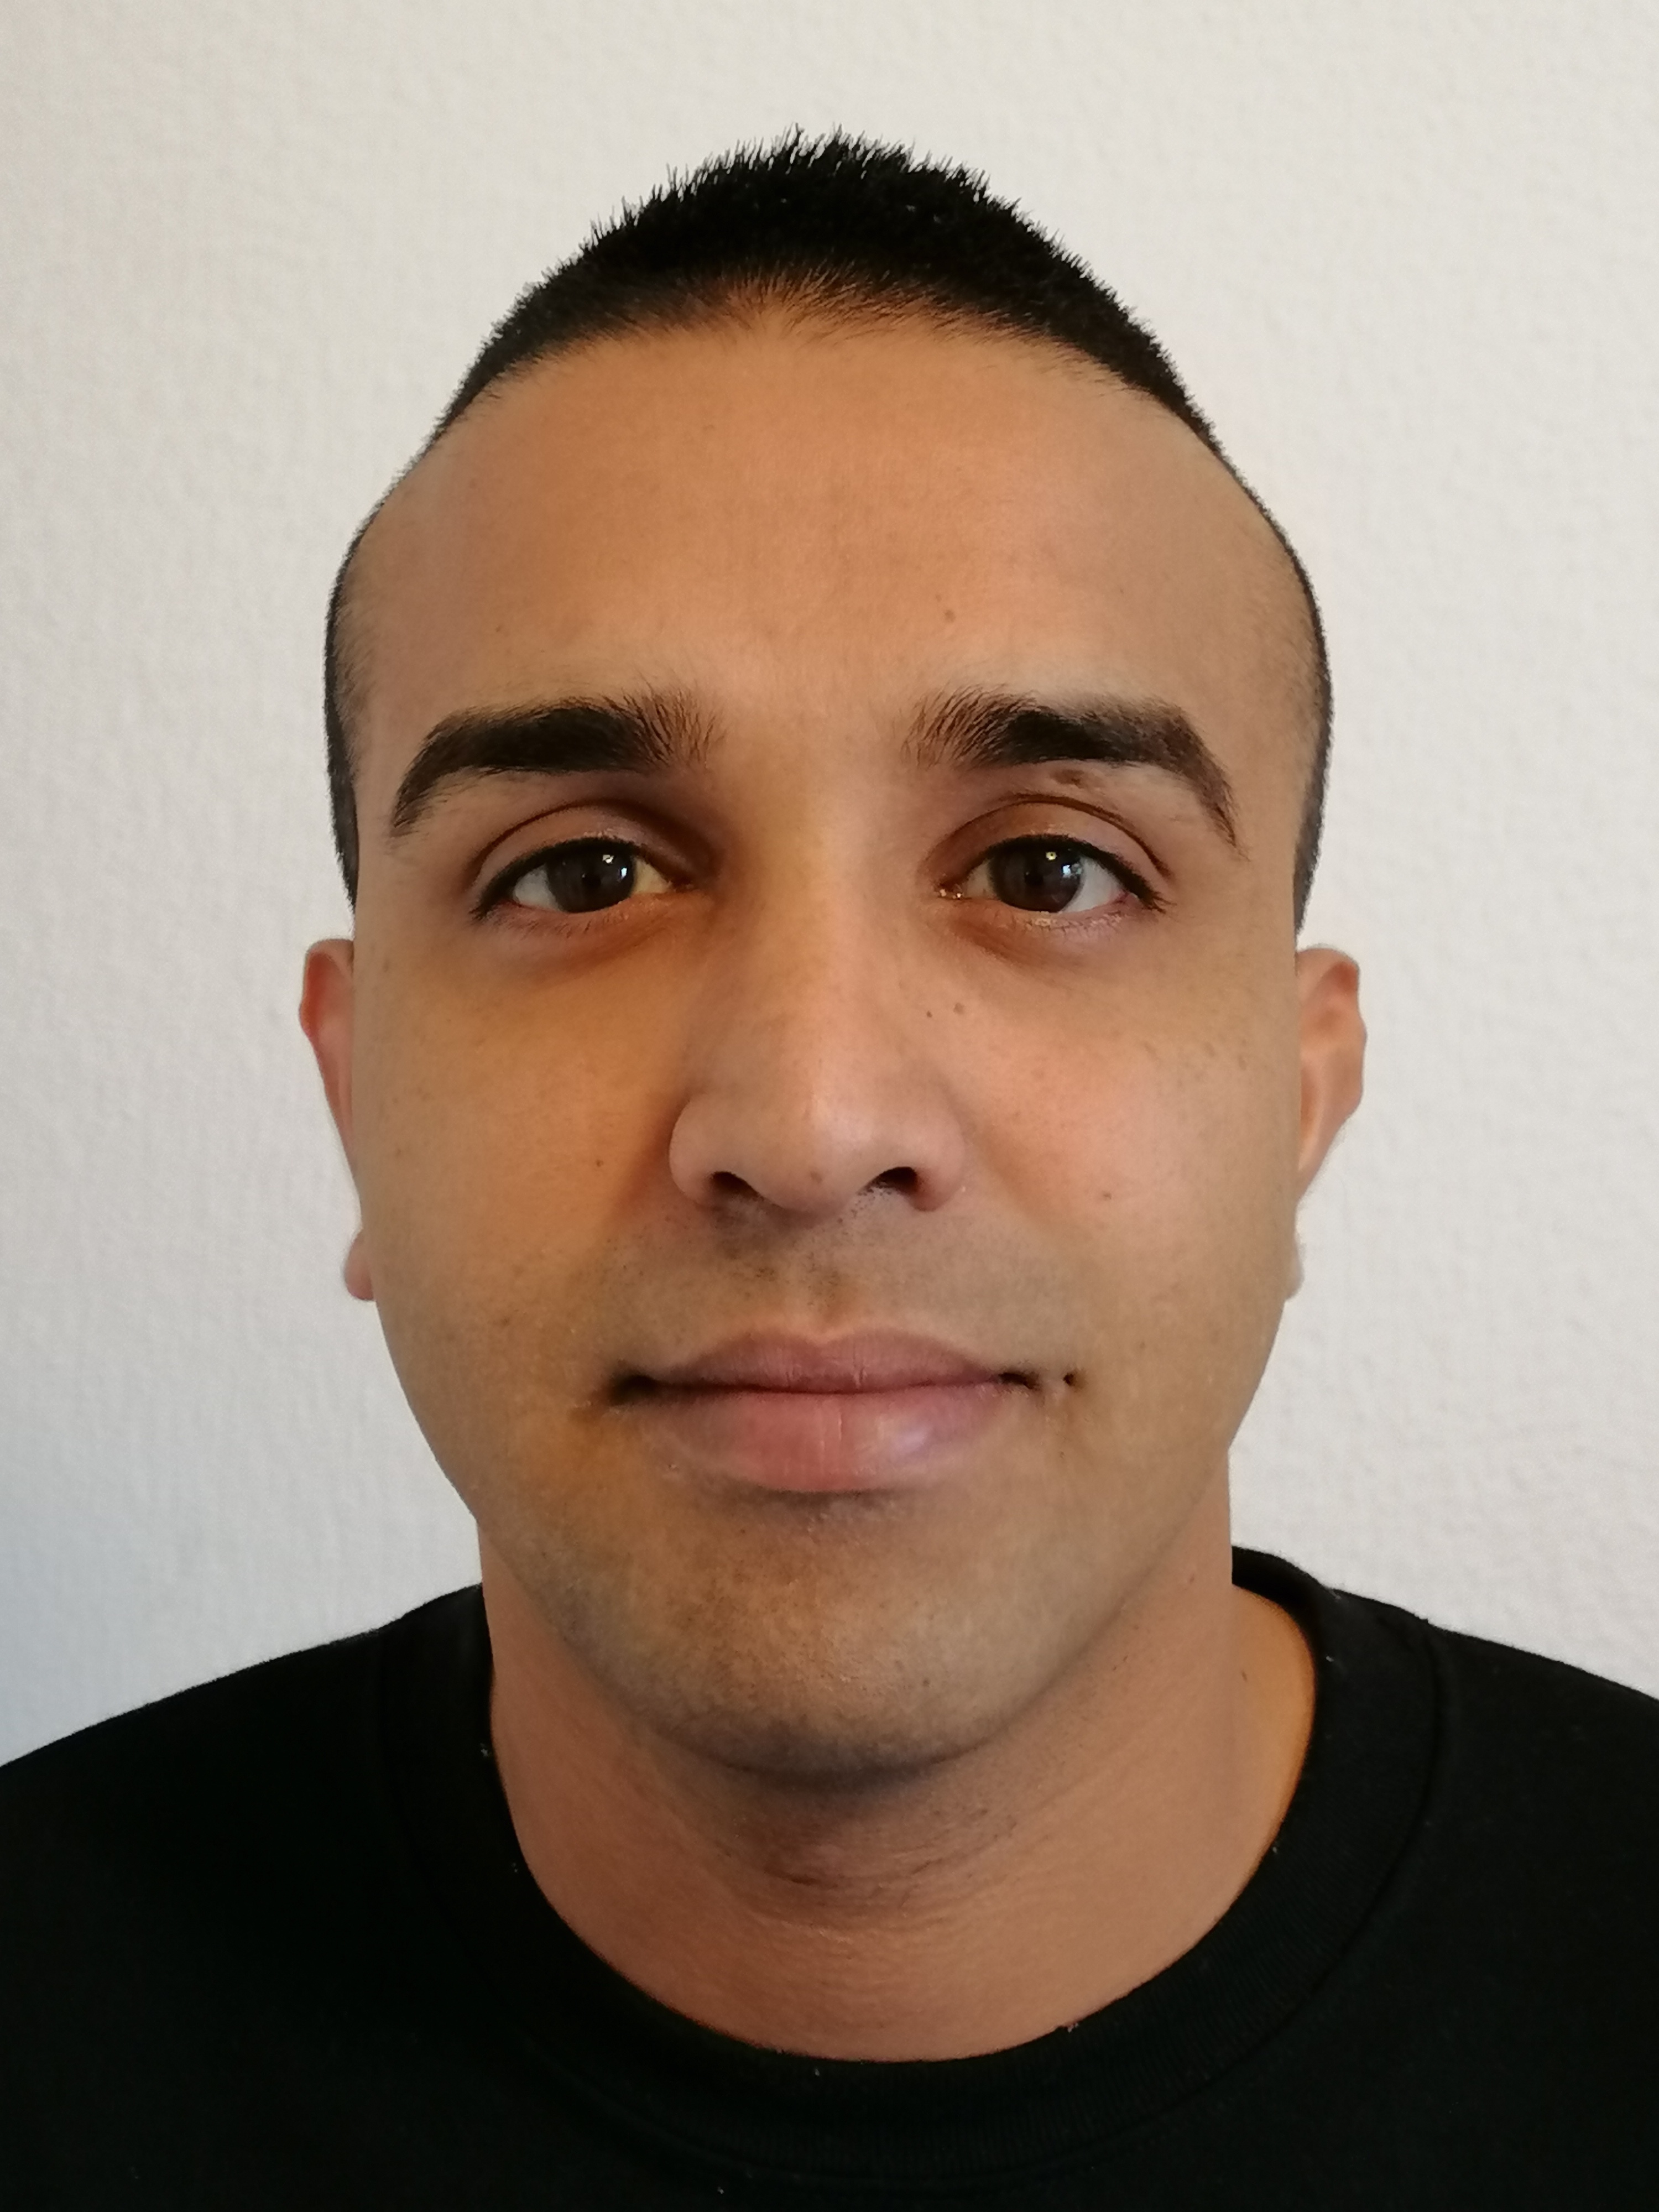
\includegraphics[width=0.65\textwidth]{foto.jpg}\hfill\null

\vspace*{0.5ex} % Extra space after the picture

\headleft{Profile Summary}
I am deeply passionate about IT and have spent years independently exploring and studying this fascinating field.

\headleft{Contact details}
\small % To fit more content
\MVAt\ {\small gurdipku91@gmail.com} \\[0.4ex]
\Mobilefone\ +41\,77\,99\,32\,80\,04 \\[0.5ex]
\Letter\ Eggen 2, 4625 Oberbuchsiten
\normalsize

\headleft{Personal information}
%Year of birth: \textbf{1861} \\[0.5ex]
Citizenship: \textbf{\textit{Italian, Indian}}\\[0.5ex]
%Family: \textbf{Married with children} \\[0.5ex]
Languages: \textbf{German}, \textbf{Italian}, \textbf{English}, \textbf{Hindi}

\headleft{Skills}
\begin{itemize}
\item Python
\item Panda, Numpy, Tkinter 
\item SQL
\item JavaScript
\item React, HTML, CSS
\item Git/GitHub
\item Cybersecurity
\item Networking
\end{itemize} 

\end{minipage}%
\kern0.09\textwidth\relax%%Right margin provided explicitly to stretch the colourbox
}
\end{minipage}% Right column
\hskip2.5em% Left margin for the white area
\begin{minipage}[t]{0.56\textwidth}
\setlength{\parskip}{0.8ex}% Adds spaces between paragraphs; use \\ to add new lines without this space. Shrink this amount to fit more data vertically

\vspace{2ex}

\headright{Experience}

\textsc{Data analyst} at \textit{XXXX (Hyderabad).}  \dates{2018.08--2024.05} \\

\smaller{Collected, cleaned, and processed large datasets from multiple sources to ensure data accuracy and integrity.}


\is
\smaller{Conducted exploratory data analysis to identify patterns, trends, and insights using statistical methods and data visualization techniques to support business decisions.}
 

\is
\smaller{Having good experience on T-SQL, Microsoft SQL Server
Management Studio. Solid knowledge of database management systems and data warehousing concepts.}

\is
\smaller{Having good knowledge creating Relationships in data model like one-one, one-many, many-one and many-many. Monitoring and validating key metrics insights data from daily report.}


\headright{Certifications}

%\smaller{\textsc{Introduction to Data Analysis using Microsoft Excel,}} \textit{Coursera.} \\
%\is
%%\smaller{\textsc{Data Analysis With Python,Cognitive Class DA0101EN,} \textit{provided by IBM.}} %\dates{July-3-2024} \\
%%\is
%%\smaller{\textsc{SQL, Hacker Rank}}

\smaller{\textbf{Machine Learning,}} \textit{Coursera.} \\
\smaller{Issued March 2024} \\
\smaller{Instructor: Andrew Ng} \is

\smaller{\textsc{Deep Learning Specialization,}} \textit{Coursera.} \\
\smaller{Issued April 2024} \\
\smaller{Instructor: Andrew Ng} \is

\smaller{\textsc{Data Science Professional Certificate,}} \textit{IBM.} \\
\smaller{Issued June 2024} \is

\smaller{\textsc{Python for Data Science, AI & Development,}} \textit{IBM.} \\
\smaller{Issued February 2024} \is

\smaller{\textsc{Introduction to Cloud Computing,}} \textit{IBM.} \\
\smaller{Issued January 2024} \is

\smaller{\textsc{Certified Information Systems Security Professional (CISSP),}} \textit{(ISC)².} \\
\smaller{Issued August 2023 · Expires August 2026} \is

\smaller\begin{itemize}
        \item \textbf{Issuer:} Craw Security
        \item \textbf{Issued:} August 2023
        \item \textbf{Skills:} Linux
    \end{itemize}


\headright{Education}

\textsc{Master of Computer Application (MCA).} \textit{from JNTU Kakinada University}. \dates{2012--2015} \\

\is
\textsc{Bachelor of Science in Mathematics, Physics, and Computer
Science.} \textit{Acharya Nagarjuna University}.  \dates{2007--2010} \\

\headright{Hobbies}

\textit{Listening Music, Playing Cricket}
\end{minipage}

\end{document}
